

\documentclass[]{article}
\usepackage[dutch]{babel}
\usepackage{listings}
\usepackage{color}
\usepackage{graphicx}
\graphicspath{/Users/alexandre/Dropbox/1eBaCW}
\title{Programmeerproject: Eindverslag Fase 3}
\author{ Alexandre Kahn \\
			alexkahn@vub.ac.be \\
			0500067 \\
			Faculteit Wetenschappen en Bio-ingenieurswetenschappen \\
			Vrije Universiteit Brussel}
\definecolor{mygreen}{rgb}{0,0.6,0}
\definecolor{mygray}{rgb}{0.5,0.5,0.5}
\definecolor{mymauve}{rgb}{0.58,0,0.82}
\lstset{ %
	backgroundcolor=\color{white},   % choose the background color; you must add \usepackage{color} or \usepackage{xcolor}
	basicstyle=\footnotesize,        % the size of the fonts that are used for the code
	breakatwhitespace=false,         % sets if automatic breaks should only happen at whitespace
	breaklines=true,                 % sets automatic line breaking
	captionpos=b,                    % sets the caption-position to bottom
	commentstyle=\color{mygreen},    % comment style
	deletekeywords={...},            % if you want to delete keywords from the given language
	escapeinside={\%*}{*)},          % if you want to add LaTeX within your code
	extendedchars=true,              % lets you use non-ASCII characters; for 8-bits encodings only, does not work with UTF-8
%	frame=single,	                   % adds a frame around the code
	keepspaces=true,                 % keeps spaces in text, useful for keeping indentation of code (possibly needs columns=flexible)
	keywordstyle=\color{blue},       % keyword style
	language=Lisp,                 % the language of the code
	otherkeywords={*,...},           % if you want to add more keywords to the set
	numbers=left,                    % where to put the line-numbers; possible values are (none, left, right)
	numbersep=5pt,                   % how far the line-numbers are from the code
	numberstyle=\tiny\color{mygray}, % the style that is used for the line-numbers
	rulecolor=\color{black},         % if not set, the frame-color may be changed on line-breaks within not-black text (e.g. comments (green here))
	showspaces=false,                % show spaces everywhere adding particular underscores; it overrides 'showstringspaces'
	showstringspaces=false,          % underline spaces within strings only
	showtabs=false,                  % show tabs within strings adding particular underscores
	stepnumber=1,                    % the step between two line-numbers. If it's 1, each line will be numbered
	stringstyle=\color{mymauve},     % string literal style
	tabsize=2,	                   % sets default tabsize to 2 spaces
	title=\lstname                   % show the filename of files included with \lstinputlisting; also try caption instead of title
}
\begin{document}
\maketitle
\date
\begin{center}
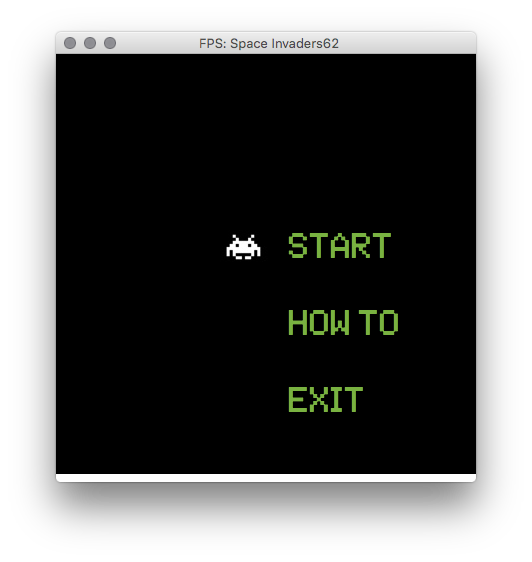
\includegraphics[scale=0.5]{Voorblad}
\end{center}
\newpage
\tableofcontents
\newpage

\section{Inleiding}
Dit is het verslag van de laatste fase. We moesten er voor zorgen dat ons spel af was. \\ 
In de vorige versie moest het spel al extra spelelementen hebben, nu moest alles er zijn. De highscore wordt bijgehouden en opgeslagen. De score en de highscore moeten op het spelbord getekend worden.  Er moeten power-ups zijn die verschillende zaken aanpassen in het spel, en na enkele seconden gedeactiveerd worden. 
\section{Abstracte Data Types}
Het schip-ADT is exact hetzelfde gebleven, het kogel-adt is licht aangepast zodat er verschillende soorten kogels kunnen bestaan. In het alien-ADT waren er ook kleine veranderingen, zo wordt er aan het vloot-ADT meegegeven dat het zich moet opkuisen als er een alien geraakt is.  De ADT's die met het menu te maken hebben zijn net als het spel-adt vooral opgekuist. Tot slot zijn er nieuwe ADT's voor de score en voor de power-ups.
\subsection{Alien-ADT}
De aliens worden allemaal apart aangemaakt en zijn objecten op hun eigen. Om er meerdere op te roepen is er het \texttt{Vloot-ADT}. \\
Elk alien-object zal zijn eigen positie hebben en bijhouden, alsook de kleur en hoeveel levens deze nog heeft. Het aantal levens is aan de kleur gelinkt. \\ 
Door elk hun eigen positie bij te houden kan het vloot-adt gemakkelijk de co\"{o}rdinaten te veranderen. 
\begin{center}
	\begin{lstlisting}
		(maak-alien-adt <x-positie> <y-posititie> <kleur> <teken-adt>)
	\end{lstlisting}

\begin{tabular}{|c|c|c|}
	\hline  \textbf{Message} & \textbf{Parameter} & \textbf{Resultaat}  \\ 
	\hline  x  & / &  Geeft de positie van het opgevraagde x-co\"{o}rdinaat terug.\\
	\hline  y  & / & Geeft de positie van het opgevraagde y-co\"{o}rdinaat terug.\\  
	\hline x! & nieuwe-x & Geeft het object een nieuwe x-positie.   \\
	\hline y! & nieuwe-y & Geeft het object een nieuwe y-positie.  \\ 
	\hline levens & / & Geeft het aantal levens terug.  \\   
	\hline levens! & getal & Past het aantal levens aan. \\   
	\hline  teken! & teken-adt & Geeft aan het teken-ADT mee dat het, het alien-object \\ && moet tekenen. \\ 
	\hline  delete! & teken-adt & Geeft aan het teken-ADT mee dat het alien-object verwijderd \\ & &moet worden. \\ 
	\hline geraakt! & kogel-adt teken-adt & Deze message neemt een leven van de alien weg. \\ &   vloot-adt score-adt  &Indien deze er geen meer heeft wordt de alien \\ &kogels-adt  huidige-tijd spel & gedeletet en de vloot opgekuist. \\
	\hline
\end{tabular} 
\end{center}
\subsection{Vloot-ADT}
Bij aanmaak van de vloot moet er meegegeven worden hoeveel aliens men moet hebben. Deze worden dan allemaal in een lijst opgeslagen. Deze begint leeg en wordt dan aangevuld met alien-objecten. Als er meer dan een bepaald aantal zijn zullen deze paars zijn, die daarna zullen groen zijn en de laatste rij is altijd geel. Momenteel is dit zodat alles zo automatisch mogelijk gebeurt.\\
Er wordt dan aangevuld tot als het maximum voor een rij bereikt wordt. Hiervoor wordt dan de \texttt{afstand-tussen-2} berekend. Voor de volgende rijen gebeurt dan hetzelfde \\
 Verder is er een functie om over de vloot te lopen, \texttt{loop-over-vloot}. Deze is zeer belangrijk voor de collision-detection, want er moet voor elke alien gekeken worden of deze geraakt wordt. \\ De beweging van de aliens wordt hier ook meegegeven. Er wordt altijd gecheckt of er een botsing gebeurt met een zijkant van het scherm en indien dit het geval is wordt de richting omgedraaid. Ook wordt er bijgehouden welk de laagste alien is en of deze de onderkant van het scherm raakt. In dat geval wordt het spel herstart. Er zijn ook functies om de vloot te versnellen en te vertragen.
 
\begin{center}
	\begin{lstlisting}
	(maak-vloot-adt <aantal> <teken-adt>)	
	\end{lstlisting}
	\begin{tabular}{|c|c|c|}
		\hline  \textbf{Message} & \textbf{Parameter} & \textbf{Resultaat}  \\
		\hline maak-aliens! & Aantal &Vult de lege lijst aan met nieuwe aliens. En laat het \\ &pos-y&teken-ADT nieuwe alien-tiles aanmaken.\\
		\hline teken! & teken-adt &Zorgt dat elk alien-object zichzelf tekent. \\
		\hline loop-over-vloot& functie & Zorgt dat een bepaalde functie gemapt wordt over \\ & &alien-objecten. \\
		\hline beweeg! & / &Zorgt dat elk alien-object zich verplaatst. \\
		\hline vloot & / & Geeft lijst met al de aliens terug. \\
		\hline verwijder-vloot! & / & Zet de lijst met alle aliens terug op null. \\
		\hline stop! & / & Pauzeert de beweging van de aliens. \\
		\hline herstart! & / &herstart de beweging van de aliens. \\
		\hline delete-dode-aliens & / & Haalt de dode aliens uit de lijst. \\
		\hline maak-alien-tiles! & / &Maakt voor elke alien een tile aan in het teken-adt. \\
		\hline
	\end{tabular}
\end{center}
\subsection{Schip-ADT}
Het schip-adt maakt een schip aan. Deze zal over de onderrand van het scherm moeten bewegen en kogels kunnen afschieten. \\
De \texttt{y-positie} zal altijd 1 zijn, de onderrand van het scherm. In het begin zal de \texttt{x-positie} steeds 0.5, of het midden van het venster zijn. De \texttt{snelheid} of het aantal stappen waarmee het schip zich zal voortbewegen is 0.3, dit zorgt voor een mooie vloeiende beweging en een gemakkelijk bestuurbaar schip. \\
De \texttt{beweeg!}-functie zal afhankelijk van de meegegeven toetsenbord-input het schip recht of links verplaatsten. Echter indien het zich al in de rand van het venster bevindt zal het niet verder bewegen, dit om te vermijden dat de raket van het spelbord zou verdwijnen.  
\begin{center}
		\begin{lstlisting}
			(maak-schip-adt)
		\end{lstlisting}
	\begin{tabular}{|c|c|c|}
		\hline  \textbf{Message} &\textbf{Parameter} & \textbf{Resultaat}  \\
		\hline  x! & nieuwe-x &Zorgt ervoor dat de x-positie van het schip aangepast wordt.\\ && Moet enkel voor x bestaan, aangezien de y-positie steeds 1 blijft.\\
		\hline x & /& Geeft de x-co\"{o}rdinaat van het schip terug. \\
		\hline beweeg! &richting & Zorgt afhankelijk van de meegegeven richting voor een \\ & &verplaatsing naar die kant. \\
		\hline teken! &teken-adt & Geeft aan het teken-adt mee om het schip te tekenen. \\
		\hline
	\end{tabular}
\end{center}
\subsection{Kogel-ADT}
Het kogel-ADT wordt niet meer vanaf het begin van het spel aangemaakt, aangezien er nu meerdere van deze ADT's zullen zijn. Ze zullen beheerd worden door een adt dat op het vloot-adt lijkt. Elke kogel zal nog steeds zijn eigen type, staat en snelheid hebben en zal ook zelf zien of het een alien raakt. Ook de beweging zit in dit ADT en zal nagaan of de kogel zich tegen een rand bevindt. 
\begin{center}
		\begin{lstlisting}
			(maak-kogel-adt posx type)
		\end{lstlisting}
	\begin{tabular}{|c|c|c|}
		\hline  \textbf{Message} & \textbf{Parameter} & \textbf{Resultaat}  \\
		\hline  x! & nieuwe-x & Zorgt ervoor dat de x-positie van de kogel aangepast wordt.\\ 
		\hline  y! & nieuwe-y& Zorgt ervoor dat de y-positie van de kogel aangepast wordt.\\
		\hline x & /&Geeft de x-co\"{o}rdinaat van de kogel terug. \\
		\hline y & /&Geeft de y-co\"{o}rdinaat van de kogel terug. \\
		\hline beweeg! & teken-adt & Zorgt voor de verplaatsing en kijkt of de kogel tegen de rand komt. \\
		\hline teken! & teken-adt&  Geeft aan het teken-adt mee om het schip te tekenen. \\
		\hline staat? & /& Geeft de staat van de kogel terug. \\
		\hline schietlus & teken-adt &Gaat na of de kogel een alien raakt. \\ & vloot-adt& en indien nodig delete deze de kogel en de alien \\
		\hline type & / & Geeft het type van de kogel terug \\
		\hline geraakt! & alien & Delete de alien, zet de kogel op inactief en geeft mee aan  \\ & alien & het teken-adt om deze te deleten \\
		\hline
	\end{tabular}
\end{center}
\subsection{Kogels-ADT}
Dit ADT zorgt om de meerdere kogels in goede banen te leiden en op een correcte manier aan te spreken. Het doel is om alle kogels in een lijst op te slaan. Dit gebeurt door telkens de nieuwe kogel voor de al bestaande te consen. Het heeft functies om een nieuwe kogel te maken, een functie om functies op alle kogels uit te voeren, zorgt ervoor dat alles getekend wordt en dat alle kogels kunnen bewegen. In de \texttt{beweeg!} functie wordt er ook nagegaan of de kogel een alien raakt. Er is ook een functie die inactieve kogels verwijderd.
\begin{center}
	\begin{lstlisting}
	(maak-kogels-adt)
	\end{lstlisting}
	\begin{tabular}{|c|c|c|}
		\hline  \textbf{Message} & \textbf{Parameter} & \textbf{Resultaat}  \\
		\hline beweeg! & teken-adt &Zorgt dat elke kogel moet bewegen en nagaan of \\ & vloot-adt & deze botst. \\
		\hline teken! & teken-adt&  Geeft aan de kogels mee dat ze zichzelf moeten tekenen. \\
		\hline maak-kogel! & posx, & Maakt een nieuw kogel-adt aan en plaatst deze in de lijst. \\ &teken-adt & Ook wordt er in het teken-adt een nieuwe kogel aangemaakt. \\
		\hline kogels & / & Geeft de lijst met kogels terug. \\
		\hline delete-inactieve-kogels & / & Haalt de inactieve kogels weg uit de lijst. \\
		\hline volgende-kogel! & type & Bepaalt het type van de volgende kogel. \\
		\hline
	\end{tabular}
\end{center}
\subsection{Teken-ADT}
Het \texttt{teken-ADT} zorgt ervoor dat alle objecten getekend worden. Het maakt hiervoor gebruik \texttt{Graphics.rkt}. \\
Bij het aanmaken van dit ADT, wordt er een venster met zwarte achtergrond getekend. Hierop komen dan verschillende lagen,\texttt{'make-layer}, voor de objecten. Deze worden op hun laag getekend als tegels, \texttt{'make-tile}. Voor het schip, het menu, de how-to en de rotator is dit simpel, er moet slechts een tegel gemaakt worden. De aliens en kogel zitten daarentegen in lijsten. Voor de beide is dit zodat er meerdere getekend kunnen worden.  \\
Zowel de kogels als de aliens zijn te verwijderen, dit door in de lijst de correcte tegel weg te halen. Dat kan aan de hand van \texttt{neem-iets}. De functie zoekt het juiste object en geeft deze dan terug. \\
Het tekenen van de tiles gebeurt bijna altijd op dezelfde manier, zo wordt indien nodig de juiste tegel gezocht, dan worden de correcte co\"{o}rdinaten berekend, de x-waarde gecentraliseerd en de tegel op deze positie getekend. \\
Er zijn ook functies die alle sprites hertekenen en verwijderen indien er bijvoorbeeld een menu getekend moet worden.
\begin{center}
	\begin{lstlisting}
	(maak-adt-teken <titel> <hoogte> <breedte>)
	\end{lstlisting}
	\begin{tabular}{|c|c|c|}
		\hline  \textbf{Message} &\textbf{Parameters} & \textbf{Resultaat}  \\
		\hline  set-toets-functie! & fun &Zorgt dat de toetsenbordinput ingelezen wordt. \\
		\hline set-spel-lus-functie! &fun & Zorgt ervoor dat het speelbord steeds geupdatet wordt. \\
		\hline teken-schip! & schip-adt &Zorgt ervoor dat het schip getekend wordt. \\
		\hline teken-alien! & alien-adt &Zorgt ervoor dat de alien getekend wordt. \\
		\hline teken-kogel! & kogel-adt &Zorgt ervoor dat de kogel getekend wordt. \\
		\hline teken-menu! & menu-adt &Zorgt ervoor dat het menu getekend wordt. \\
		\hline teken-rotator! & rotator-adt &Zorgt ervoor dat de rotator getekend wordt. \\
		\hline teken-how-to! & how-to-adt &Zorgt ervoor dat de how-to getekend wordt. \\
		\hline teken-score! & score-adt &Zorgt ervoor dat de score en high-score getekend worden. \\
		\hline teken-power-up! & power-up-adt & Zorgt ervoor dat de power-up getekend wordt. \\
		\hline herteken-spelelementen & / & Zorgt dat alle spelementen hertekend worden. \\
		\hline nieuwe-alien! & alien-adt & Maakt een nieuwe alien-tile en voegt deze toe aan de lijst. \\
		\hline nieuwe-kogel! & kogel-adt &  Maakt een nieuwe kogel-tile en voegt deze toe aan de lijst.\\
		\hline maak-rotator! &rotator-adt& Voegt de rotator-tile toe aan de laag. \\
		\hline maak-menu! &menu-adt& Voegt de menu-tile toe aan de laag. \\
		\hline maak-how-to &how-to-adt& Voegt de how-to-tile toe aan de laag. \\
		\hline delete-alien! & alien-adt & Zoekt de correcte alien-tile en verwijderd deze. \\
		\hline delete-kogel! & kogel-adt & Zoekt de correcte kogel-tile en verwijderd deze. \\
		\hline delete-schip! & / & Delete de schip-tile van het scherm. \\
		\hline delete-menu! & / & Delete de menu-tile van het scherm. \\
		\hline delete-rotator! & / & Delete de rotator-tile van het scherm. \\
		\hline delete-how-to! & / & Delete de how-to-tile van het scherm. \\
		\hline delete-power-up! & / & Delete de power-up-tile van het scherm. \\
		\hline verwijder-spelelementen & / & Delete het schip, alle aliens en alle kogels. \\ 
		\hline reset-vloot! & / & Haalt alle aliens weg uit de vlootlijst, haalt ook de tiles weg \\
		\hline voeg-alien-tile-toe! & alien-adt& Voegt de tile, die bij het correcte ADT hoort toe. \\
		\hline 
	\end{tabular}
\end{center}
\subsection{Spel-ADT}
Dit ADT bevat de eigenlijke spellus. Er is de functie, \texttt{start} om het spel te starten. Verder zijn er \texttt{pauze}, om het spel te pauzeren en het menu te tekenen, \texttt{play}, om de gameloop te starten, \texttt{howto}, om de tutorial te tonen en \texttt{nieuw-level} om een nieuw level te starten. 
Er is een \texttt{spel-lus-functie-play} voor de spellus en ook een \texttt{spel-lus-functie-pauze} die niets doet, voor in het menu. Verder zijn er \texttt{toets-naar-spel}-functies voor zowel de spellus, het menu, als de how-to pagina. \\

\begin{center}
	\begin{lstlisting}
	(maak-adt-spel)
	\end{lstlisting}
	\begin{tabular}{|c|c|c|}
		\hline  \textbf{Message} &\textbf{Parameter} & \textbf{Resultaat}  \\
		\hline start & / & Dit is de entry point die ervoor zorgt dat de spellus en hierbij het \\ & & hele spel start. \\
		\hline pauze! & / & Zet het spel op pauze. \\
		\hline restart! & / & Pauzeert het spel, delete de aliens en maakt er nieuwe aan. \\
		\hline nieuw-level! & / & Verhoogt het level en maakt meer en nieuwe aliens aan. \\
		\hline 
	\end{tabular}
\end{center}
\subsection{Menu-ADT}
Dit ADT dient om het menu weer te geven en is zeer simpel. Het heeft een vaste positie en moet instaat zijn het menu te installeren, dit is alle spelelementen weghalen en het menu te tekenen, als het omgekeerde bij het \texttt{uninstall} commando. Ook houdt het de staat van het spel bij. \\
\begin{center}
	\begin{lstlisting}
	(maak-menu-adt)
	\end{lstlisting}
	\begin{tabular}{|c|c|c|}
		\hline  \textbf{Message} &\textbf{Parameter} & \textbf{Resultaat}  \\
		\hline x & /&Geeft de x-co\"{o}rdinaat van het menu terug. \\
		\hline y & /&Geeft de y-co\"{o}rdinaat van het menu terug. \\
		\hline teken! &teken-adt& Laat het teken-adt weten dat het menu getekend moet worden. \\
		\hline staat & / & Geeft de staat van het spel terug. \\
		\hline staat! & nieuwe-staat & Verandert de staat naar de nieuwe staat.	\\
		\hline delete! & teken-adt & Verwijdert het menu uit het teken-adt. \\
		\hline install! & teken-adt & Haalt de spelelementen weg en maakt het menu aan. \\
		\hline uninstall& teken-adt & Delete het menu en hertekend de spelelementen. \\
		\hline 
	\end{tabular}
\end{center}
\subsection{Rotator-ADT}
Dit ADT dient voor de selector in het menu. Het moet ook niet veel kunnen, behalve op de correcte posities verschijnen. Hiervoor heeft het ook een staat zodat het spel gemakkelijk kan weten welke keuze er gemaakt wordt. 
\begin{center}
	\begin{lstlisting}
	(maak-menu-adt)
	\end{lstlisting}
	\begin{tabular}{|c|c|c|}
		\hline  \textbf{Message} &\textbf{Parameter} & \textbf{Resultaat}  \\
			\hline x & /&Geeft de x-co\"{o}rdinaat van de rotator terug. \\
			\hline y & /&Geeft de y-co\"{o}rdinaat van de rotator terug. \\
			\hline teken! &teken-adt& Laat het teken-adt weten dat de rotator getekend moet worden. \\
			\hline staat & / & Geeft de staat van de rotator terug. \\
			\hline up! & / & Doet de rotator stijgen, indien het kan en verandert de staat. \\ 
			\hline down! & / & Doet de rotator dalen, indien het kan en verandert de staat. \\ 
		\hline
		\end{tabular}
	\end{center}
\subsection{How-To-ADT}
Dit ADT dient om de controls te tonen. Moet ook heel weinig kunnen. Hier zijn ook een \texttt{install!} en \texttt{uninstall!} functie gemaakt om de correcte dingen van het scherm te halen of juist te tonen. 
\begin{center}
	\begin{lstlisting}
	(maak-menu-adt)
	\end{lstlisting}
	\begin{tabular}{|c|c|c|}
		\hline  \textbf{Message} &\textbf{Parameter} & \textbf{Resultaat}  \\
		\hline x & /&Geeft de x-co\"{o}rdinaat van de How-To terug. \\
		\hline y & /&Geeft de y-co\"{o}rdinaat van de How-To terug. \\
		\hline  teken! &teken-adt& Laat het teken-adt weten dat de How-To getekend moet worden. \\
		\hline install! & teken-adt& Delete het menu en tekent de how-to. \\
		\hline uninstall! & teken-adt & Delete de how-to en tekent het menu. \\
		\hline 
		\end{tabular}
	\end{center}\
\subsection{Power-Up-ADT}
Dit ADT dient om Power-ups aan te maken. Ze worden op random plaatsen getekend en maken gebruik van timers om te weten wanneer en hoe lang ze mogen verschijnen.
\begin{center}
	\begin{lstlisting}
(maak-power-up-adt positie-x positie-y teken-adt)
	\end{lstlisting}
	\begin{tabular}{|c|c|c|}
		\hline  \textbf{Message} &\textbf{Parameter} & \textbf{Resultaat}  \\
		\hline x & /&Geeft de x-co\"{o}rdinaat terug. \\
		\hline y & /&Geeft de y-co\"{o}rdinaat terug. \\
		\hline kleur & /&Geeft dekleur terug. \\
		\hline levens & /&Geeft het aantal levens terug. \\
		\hline staat & /&Geeft de staat terug. \\
		\hline timer & /&Geeft de timer levens terug. \\
		\hline reset! & /&Reset het object. \\
		\hline activeer! & /&Activeert het object en geeft het de correcte kleur. \\
		\hline deactiveer! & /&Deactiveert het object. \\
		\hline random-nummer & /&Geeft het gegeneerde random nummer terug. \\
		\hline x! & pos-x &Verandert de x-co\"{o}rdinaat. \\
		\hline y !& pos-y &Verandert de y-co\"{o}rdinaat. \\
		\hline  teken! &teken-adt& Laat het teken-adt weten dat de power-up getekend  \\ &&moet worden. \\
		\hline geraakt! & kogel-adt teken-adt &  Zorgt dat het correcte effect gebeurt. Start \\
								& vloot-adt score-adt & een timer en zet de staat op bezig. \\
								&kogels-adt huidige-tijd spel & \\
		\hline zet-terug! &vloot-adt kogels-adt & Maakt het effect ongedaan. \\
		\hline 
	\end{tabular}
\end{center}
\subsection{Score-ADT}
Dit ADT dient om de score te tonen. Ook wordt de high-score bijgehouden en getoond.

\begin{center}
	\begin{lstlisting}
	(maak-menu-adt)
	\end{lstlisting}
	\begin{tabular}{|c|c|c|}
		\hline  \textbf{Message} &\textbf{Parameter} & \textbf{Resultaat}  \\
		\hline x & /&Geeft de x-co\"{o}rdinaat terug. \\
		\hline y & /&Geeft de y-co\"{o}rdinaat terug. \\
		\hline score & /&Geeft de score terug. \\
		\hline high-score & /&Geeft de high-score terug. \\
		\hline verhoog & getal & Maakt de nieuwe score aan en slaagt deze op indien nodig \\
		\hline  teken! &teken-adt& Laat het teken-adt weten dat het object getekend moet worden. \\
		\hline 
	\end{tabular}
\end{center}\
\begin{samepage}
\section{Afhankelijkheidsdiagram}
\begin{center}
\includegraphics[scale=0.45]{AfhankelijkheidsDiagramFase3}
\end{center}
\end{samepage}

\section{Verloop}
Een aantal zaken in deze fase verliepen zeer vlot. Zo waren de power-ups snel en gemakkelijk te implementeren, ook met de scores had ik geen problemen. Waar ik heel lang op heb zitten zoeken was hoe ik het spel moest laten herstarten, nadat de aliens de onderkant van het spelvlak raken. Aan de basis van dit probleem lag een mijn slordige code als ook een klein foutje in een for-each. Heb op aanraden van de assistenten dan mijn code wat proberen op te kuisen en zo de bug gevonden.

\section{Broncodes}

\subsection{Abstracties.rkt}
\lstinputlisting[language=Lisp]{Abstracties.rkt}
\subsection{Alien.rkt}
\lstinputlisting[language=Lisp]{Alien.rkt}
\subsection{Howto.rkt}
\lstinputlisting[language=Lisp]{howto.rkt}
\subsection{Kogel.rkt}
\lstinputlisting[language=Lisp]{Kogel.rkt}
\subsection{Kogels.rkt}
\lstinputlisting[language=Lisp]{Kogels-adt.rkt}
\subsection{Menu.rkt}
\lstinputlisting[language=Lisp]{Menu.rkt}
\subsection{Rotator.rkt}
\lstinputlisting[language=Lisp]{rotator.rkt}
\subsection{Schip.rkt}
\lstinputlisting[language=Lisp]{Schip.rkt}
\subsection{Spel.rkt}
\lstinputlisting[language=Lisp]{Spel.rkt}
\subsection{Teken-adt.rkt}
\lstinputlisting[language=Lisp]{teken-adt.rkt}
\subsection{Vloot.rkt}
\lstinputlisting[language=Lisp]{vloot.rkt}
\subsection{Power-Ups-adt}
\lstinputlisting[language=Lisp]{Power-Ups.rkt}
\subsection{Score}
\lstinputlisting[language=Lisp]{score.rkt}

\section{Bibliografie}
Sussman G.J. Abelson, A. \textit{Structure and Interpretation of Computer Programs}, The MIT Press, 1996. \\
\texttt{https://docs.racket-lang.org/reference/strings.html} \\
\texttt{http://docs.racket-lang.org/reference/file-ports.html?q=do}
\end{document}         


